% Copyright (C)  2015  Alexander Jankowski, Philipp Hacker.
% Permission is granted to copy, distribute and/or modify this document
% under the terms of the GNU Free Documentation License, Version 1.3
% or any later version published by the Free Software Foundation;
% with no Invariant Sections, no Front-Cover Texts, and no Back-Cover Texts.
% The lincense itself can be found at <https://www.gnu.org/licenses/fdl-1.3>.

\documentclass[numbers=noenddot,a4paper,notitlepage,twoside,BCOR15mm]{scrartcl}
%\documentclass[numbers=noenddot,12pt,a4paper]{scrartcl}

\usepackage{ifoddpage}
\usepackage[infoshow]{tabularx}
\usepackage{fancyhdr}
\usepackage[greek,ngerman]{babel}
\usepackage[T1]{fontenc}
\usepackage[utf8]{inputenc}
\usepackage{libertine}
\usepackage{ziffer}
\usepackage{graphicx}
\usepackage{units}
\usepackage[infoshow]{tabularx}
\usepackage[all]{xy}
\usepackage{amsmath}
\usepackage{amssymb}
\usepackage{wrapfig}
\usepackage{upgreek}
\usepackage{esint}
\usepackage{float}
\usepackage[font=small,labelfont=bf]{caption}
\usepackage{subcaption}
\usepackage{lscape}
\usepackage[backref=page]{hyperref}
\usepackage{cleveref}
\usepackage{csquotes}

\renewcommand{\headrulewidth}{0.1pt}
\renewcommand{\footrulewidth}{0.1pt}
\newcommand{\name}{\text{Alexander Jankowski}} 

\renewcaptionname{ngerman}{\figurename}{Abb. }
\renewcaptionname{ngerman}{\tablename}{Tab.}

\setlength{\parindent}{0pt}

\newcommand{\nummat}[1]{\left[\text{#1}\right]}
\newcommand{\num}[1]{$\left[\text{#1}\right]$}
\newcommand{\degree}{^\circ}
\newcommand{\diff}{\textnormal{d}}
\newcommand{\tenpo}[1]{ 10^{#1}}
\newcommand{\greek}[1]{\greektext#1\latintext}
\newcommand{\ix}[1]{_\text{#1}}
\newcommand{\imag}{\mathbf{i}}
\newcommand{\tilt}[1]{\textit{#1}}
\newcommand{\grad}[1]{\textit{grad}\left(#1\right)}
\newcommand{\divergenz}[1]{\textit{div}\left(#1\right)}
\newcommand{\euler}{\mathnormal{e}}
\newcommand{\fett}[1]{\textbf{#1}}
\newcommand{\einnup}{\hspace{0.2cm}}
\newcommand{\einnum}{\hspace{-0.2cm}}
\newcommand{\zentriert}[1]{\begin{center}#1\end{center}}

\title{Protokoll: Reflektron} 
\author{Alexander Jankowski, Philipp Hacker}
\date{\today}
\pagestyle{fancy}
\fancyhead[C]{\thepage}
\fancyhead[R]{\name}
\fancyfoot[C]{\thepage}
\fancyhead[L]{Abschnitt \thesection}

\begin{document}
	\maketitle
	\begin{center}
		Betreuer: M. Rosenbusch \\ 
		Versuchsdatum: 04.11.15\\ 
		\begin{table}[h]
			\centering
			Note:
			\begin{tabularx}{1.5cm}{|X|}
				\hline \\ \\
				\hline
			\end{tabularx}
		\end{table}
	\end{center}
	\vspace*{\fill}
	\tableofcontents
	\vfill
	\newpage
	\section{Motivation}
	
	Das Prinzip der Massenspektrometrie wird in der Physik schon lange und erfolgreich angewandt. Im Jahre 2013 beispielsweise ist es dem Experiment ISOLTRAP am CERN gelungen erstmals die Masse des äußerst kurzlebigen Isotops Zink-82 zu bestimmen mit Hilfe eines Präzisions-Flugzeit-Massenspektrometer und hat dadurch einen Einblick in die Beschaffenheit der äußeren Kruste von Neutronensternen liefern können. In diesen Versuch wird in einem kleinen Maßstab ein Teil dieser präzisen Messapparatur nachempfunden. Mit Hilfe dieses sogenannten Multireflektrons ist es möglich die Flugstrecke von Ionen und somit die Massenauflösung eines Flugzeit-Massenspektrometers von wenigen Metern auf potentiell mehreren Kilometern zu erhöhen ohne dabei die Messanlage vergrößern zu müssen. Mit Hilfe dieses Aufbaues können bereits kernphysikalische Effekte wie der Massendefekt erfolgreich aufgelöst werden.
	
	\newpage
	\section{Physikalische Grundlagen}
	
		\subsection{Flugzeit-Massenspektrometrie}
		
		Die Flugzeit-Massenspektrometrie (eng. time of flight mass sprectrometrie, kurz ToF-MS) ermöglicht es Ionen einer Probensubstanz auf ihr Masse-zu-Ladungsverhältnisses $m/q$ voneinander zu trennen und zu identifizieren. Die Trennung der Ionen erfolgt hierbei zeitlich und nicht örtlich, wie es bei anderen Varianten der Massenspektrometrie üblich ist. Im einfachsten Fall werden Ionen in einer Quelle erzeugt, anschließend mit Hilfe elektrischer Felder beschleunigt und über eine feldfreie Driftstrecke der Länge $D$ auf einen Analysator transferiert und fokussiert. Die zeitliche Trennung der Ionen erfolgt durch die zeitgleiche Beschleunigung der Ionen im elektrischen Feld $E$. Dabei nehmen alle Ionen auf der Beschleunigungsstrecke $d$ eine kinetische Energie 
		\begin{equation}
			E_\mathrm{kin}= \frac{m}{2}v^2 = qU
		\end{equation}
		auf. Demnach haben Ionen mit größerer Massen $m$ und gleicher Ladung $q$ eine kleinere Geschwindigkeit $v$ und folglich eine längere Flugzeit $t$. Bei einer konstanten Ladung ergibt sich die Relation
		\begin{equation}
		\label{eq:ToF_rel}
			t^2 \sim m.
		\end{equation}
		Eine wichtige Kenngröße eines Massenspektrometers ist das Massenauflösungsvermögen $R$. Diese gibt an wie groß der Massenabstand $\Delta m$ von einer Masse $m$ sein muss um zwei Massen unterscheiden zu können. Das Auflösungsvermögen ist definiert durch
		\begin{equation}
			R = \frac{m}{\Delta m}.
		\end{equation}
		Hierbei kann $\Delta m$ auf verschiedene Arten definiert werden, doch in der Regel wird die Halbwertsbreite des gemessenen Signals bei der Masse $m$ angegeben (eng. full with half maximum, kurz FWHM). Für ein Flugzeit-Massenspektrum kann das Auflösungsvermögen in ein Zeitauflösungsvermögen
		\begin{equation}
			R  = \frac{t}{2 \Delta t}
		\end{equation}
		transformiert werden.
		
		\subsection{Kalibrierung}
		
		Die Bestimmung der Masse mit Hilfe eines ToF-Massenspekrums ist im einfachsten Fall gegeben durch
		\begin{equation}
			m = 2qU\left(\frac{t}{D}\right)^2.
		\end{equation}
		Im allgemeinen ist die Lösung jedoch komplizierter und nicht analytisch, je nach Aufbau der Apparatur. Zur Massenbestimmung wird deshalb eine Kalibrierung des Systems mit zwei bekannten Massen $m_1, m_2$ vorgenommen. Für beide Massen kann ein Flugzeitspektrum mit zwei verschiedenen Zeiten $t_1, t_2$ aufgenommen werden. Nach \eqref{eq:ToF_rel} kann nun für die Flugzeit $t$ ein Ansatz einer linearen Gleichung in $\sqrt{m}$ angenommen werden mit den Koeffizienten $a$ und $b$. Daraus ergibt sich für die beiden Flugzeiten
		\begin{align}
			t_1 =& a\sqrt{m_1} + b, \nonumber \\
			t_2 =& a\sqrt{m_2} + b.
		\end{align}
		Die Lösung dieses linearen Gleichungssystems liefert die Koeffizienten
		\begin{align}
			a =& \frac{t_1 - t_2}{\sqrt{m_1}-\sqrt{m_2}}, \nonumber \\
			b =& \frac{1}{2}\left(t_1+t_2-\frac{\sqrt{m_1}+\sqrt{m_2}}{\sqrt{m_1}-\sqrt{m_2}}(t_1-t_2)\right).
		\end{align}
		Für eine beliebige unbekannte Masse $m$ mit der Flugzeit $t$ folgt
		\begin{equation}
			\sqrt{m} = C_\mathrm{ToF}\cdot \Delta_\mathrm{ref}+\frac{\Sigma_\mathrm{ref}}{2}
			\label{eq:masse}
		\end{equation}
		mit
		\begin{align}
			C_\mathrm{ToF} =& \frac{2t-t_1-t_2}{2(t_1-t_2)},\nonumber \\
			\Delta_\mathrm{ref} =& \sqrt{m_1}-\sqrt{m_2}, \\
			\Sigma_\mathrm{ref} =& \sqrt{m_1}+\sqrt{m_2}. \nonumber
			\label{eq:kal}
		\end{align}
		
		\subsection{Reflektron und Multireflektron}
		
		Die Ionen, welche aus der Quelle in die Driftstrecke beschleunigt werden, weisen eine nicht diskrete Energieverteilung auf, das sie zum Zeitpunkt der Beschleunigung nicht in einen Raumpunkt zentriert sind und somit durch das elektrische Feld verschiedene Beschleunigungsspannungen wahrnehmen. Ein Weg diese Energieunschärfe zu beheben und gleichzeitig die Flugstrecke des ToF-MS zu vergrößern bietet das sogenannte Reflektron. Es besteht aus einer Anordnung von Elektrodenringen, welche auf verschiedene Spannungen gelegt werden um einen Ionenspiegel zu realisieren. Der Spannungsverlauf ist so gewählt, dass Teilchen mit gleichen Massen und unterschiedlichen Energien, unterschiedlich tief in das Reflektron eindringen, bevor sie an der Potentialwand reflektiert werden. Schnellere Teilchen haben hierbei längere Wegstrecken, wodurch die verschiedenen Massen räumlich in einem Punkt fokussiert werden können.\\
		
		\begin{figure}[!h]
			\centering
			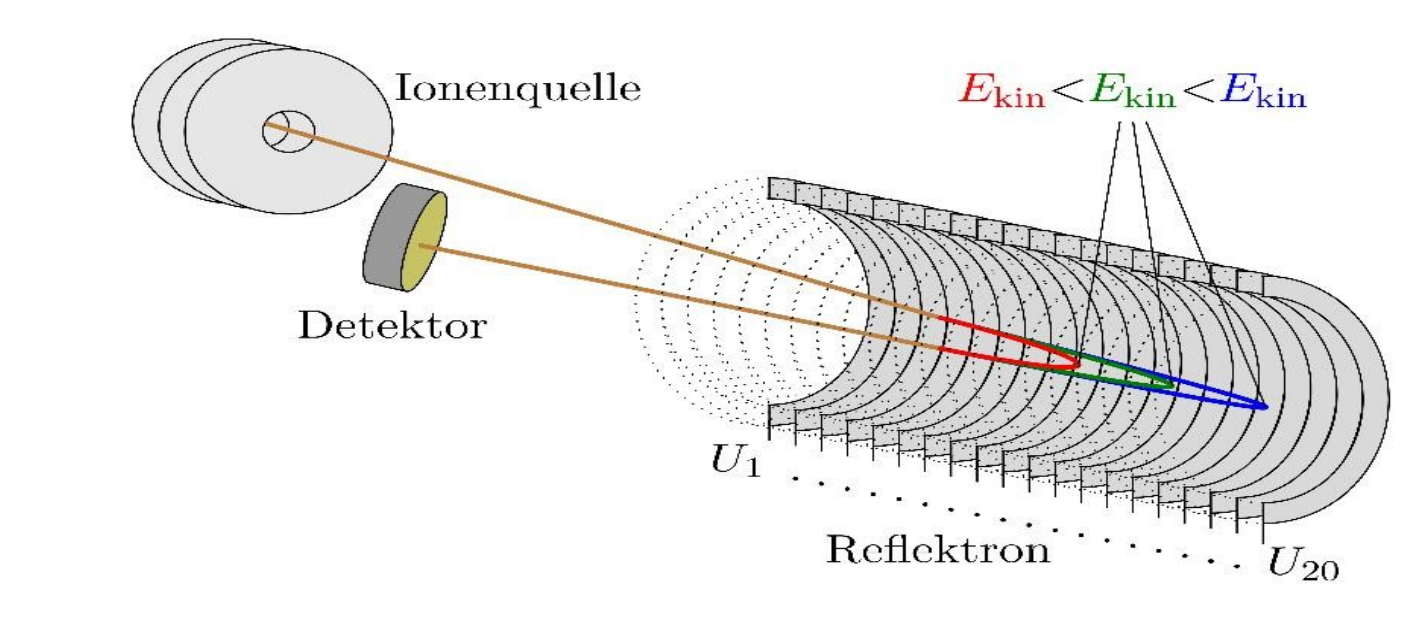
\includegraphics[width=0.8\columnwidth]{pics/Reflektron}
			\caption{Schematische Darstellung der Funktionsweise eines Reflektrons in einem ToF-MS-Aufbau.}
		\end{figure}
		In diesem Versuch wird eine statische Ionenfalle bestehend aus zwei einfachen Reflektrons verwendet um Multireflexions-Flugzeit-Massenspektrometrie (MR-ToF-MS) zu ermöglichen. Ionen, welche in dem Multireflektron gespeichert sind, bewegen sich periodisch zwischen den Spiegeln und erhöhen dadurch ihre Flugstrecke und -zeit um ein vielfaches. Dies erhöht wiederum die Massenauflösung. der Einfang und Ausschuss der Ionen aus dem Multireflektron erfolgt über eine, zwischen den Ionenspiegeln angebrachte Liftröhe, welche das durch eine quasigradientenfreie Potentialänderung die relative Energiedifferenz zwischen den der kinetischen Energie der Ionen und der Potentialwand erhöht, um die Ionen zu speichern, oder verringert um sie zu extrahieren. Um Ionen mit verschiedenen Massen $m_1, m_2$ und verschiedenen Energien $E_1, E_2$ im Multireflektron zu speichern, müssen die Ausmaße der Apparatur entsprechend gewählt werden
		\begin{equation}
			\frac{v_1}{v_2} = \sqrt{\frac{E_1}{E_2}\frac{m_2}{m_1}}< \frac{a+s+d}{a+s}.
		\end{equation}
		Hierbei sind $a$, $s$ und $d$ analog zu Abb.\ref{abb:multiref} gewählt.
		
		\begin{figure}[h]
			\centering
			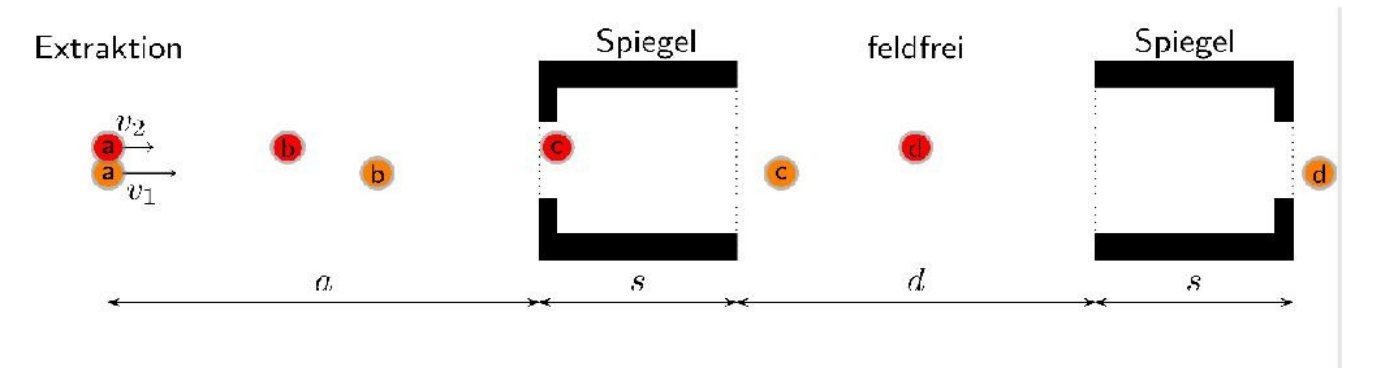
\includegraphics[width=1\columnwidth]{pics/Multireflektron}
			\caption{Schematischer Aufbau eines Multireflektrons in einem ToF-MS-Aufbau.}
			\label{abb:multiref}
		\end{figure}

		
	\newpage
	\section{Durchführung}
		
		Für den Versuch wird eine Ionenquelle verwendet, welche mit Hilfe von Ionenstoßionisation und dem Restgas in der Vakuumanlage u.a. $O_2^+$,$N_2^+$ und $N_2H^+$ Ionen erzeugen. Diese werden in einer Radiofrequenz-Falle akkumuliert und anschließend über eine Beschleunigungsstrecke in den Transferbereich extrahiert, wo diese mit Hilfe eines Liftes in das Multireflektron transferiert werden. Nach einer variablen Zeit im Multireflektron werden die Ionen extrahiert und auf einem Detektor abgebildet.
		Die Datenaufnahme und Experimentsteuerung geschieht über ein Kontrollsystem. Für die erste Messung wird ein Spektrum ohne Reflektron aufgenommen um das Signal zu prüfen. Im nächsten Schritt wird über Variation der Speicherzeit im Multireflektron die Umlaufzeit für die erzeugten Ionensorten bestimmt. Dafür wird die Zeit solange variiert, bis die Zeitabweichung zwischen $1$ Periode und $100$ Perioden minimal wird.
		Anschließend werden jeweils drei Spektren für die Umlaufzeiten der verschiedenen Ionensorten bei $100$ Umläufen aufgenommen. 
		
				\begin{figure}[h]
					\centering
					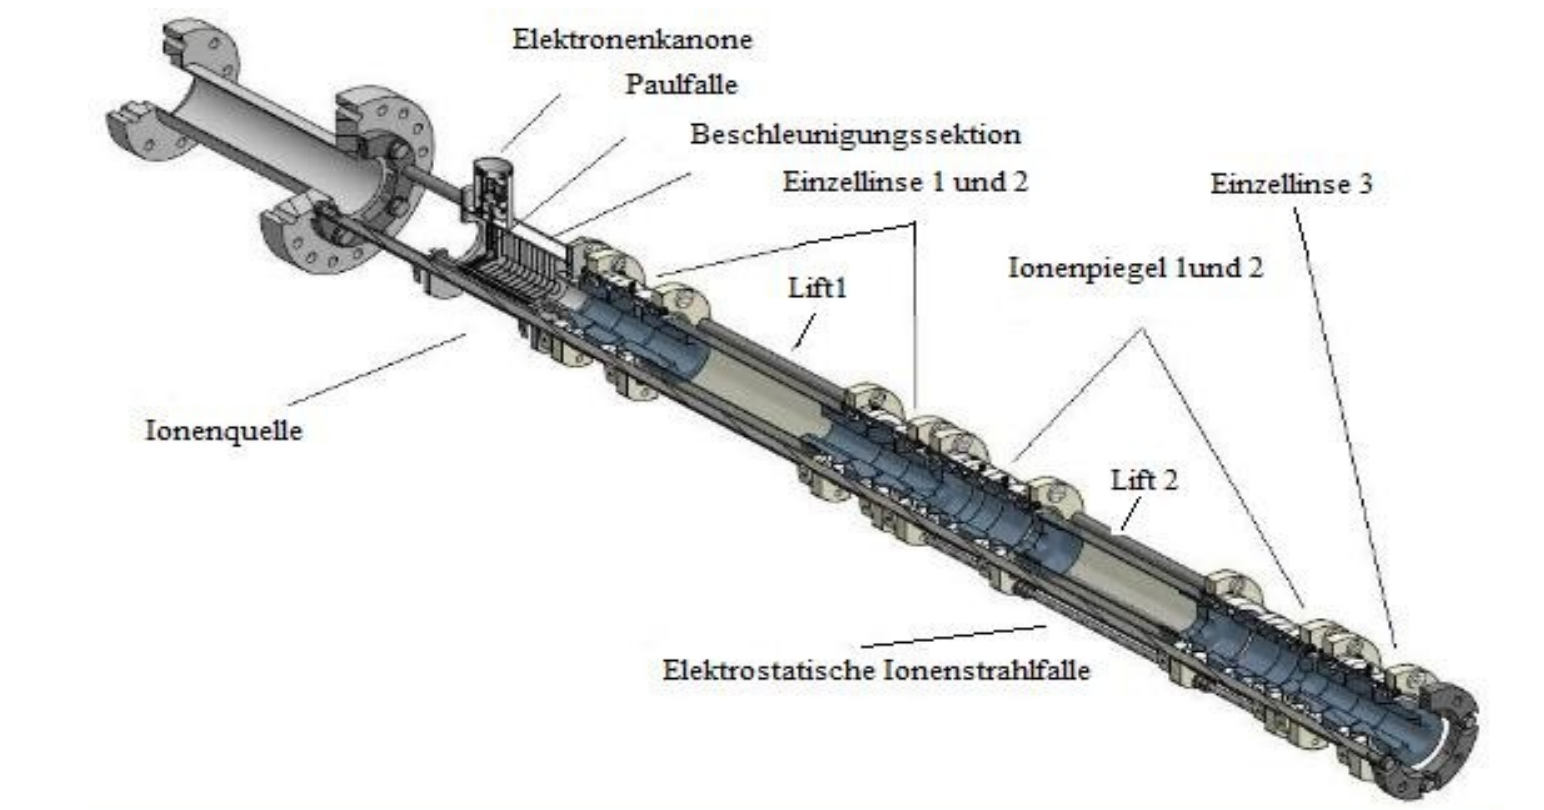
\includegraphics[width=1\columnwidth]{pics/Aufbau}
					\caption{Schematische Darstellung des Versuchsaufbaus.}
					\label{abb:aufbau}
				\end{figure}
				
		
	\newpage
	\section{Auswertung}
	
	\subsection{Bestimmung der Umlaufzeiten der Ionensorten}
	
		Um die verbesserte Massenauflösung des Multireflektrons nutzen zu können, muss zuerst die Umlaufzeit $t_\mathrm{U}$ der einzelnen Ionensorten bestimmt werden. Die Umlaufzeit gibt an wie lange das Ion braucht um eine volle Periode im Multireflektron zu vollführen. Hierfür wird die Schaltdauer des Liftes zwischen den Ionenspiegeln solange variiert, bis das Ionensignal wieder auf dem Detektor gemessen wird. Es wird ein Signalpeak betrachtet und seine Position notiert. Für die nächste Messung wird die Liftzeit Schrittweise um das $n$-fache erhöht, so dass die Ionen im Reflektron weitere Perioden vollführen. Wurde die Zeit richtig gewählt, so verschiebt sich der Peak im Flugzeitspektrum bei mehreren Perioden nicht. Ist dies doch der Fall wird die Liftzeit angepasst, bis das Signal bei $100$ Umläufen noch an der selben Stelle im Flugzeitspektrum ist. Dies wird für die Ionen N$_2^+$, O$_2^+$ und N$^2$H$^+$ durchgeführt. Die Umlaufzeiten sind in Tab.\ref{tab:umlauf} dargestellt. Die Abb.\ref{abb:N2}-\ref{abb:N2H} zeigen ein Spektrum der jeweiligen Ionensorte.
		
		\begin{table}[h]
			\centering
			\caption{Die gemessenen Umlaufzeiten $t_\mathrm{U}$ für verschiedenen Ionensorten.}
			\begin{tabular}{c|c c c}
				Ionensorte & N$_2^+$ & O$_2^+$ & N$_2$H$^+$  \\ \hline
				$t_\mathrm{U}\, /\,\mathrm{\mu s}$ & 7,265 & 7,769 & 7,3985 \\ 
			\end{tabular}
			\label{tab:umlauf}
		\end{table}
		
				\begin{figure}[h]
					\centering
					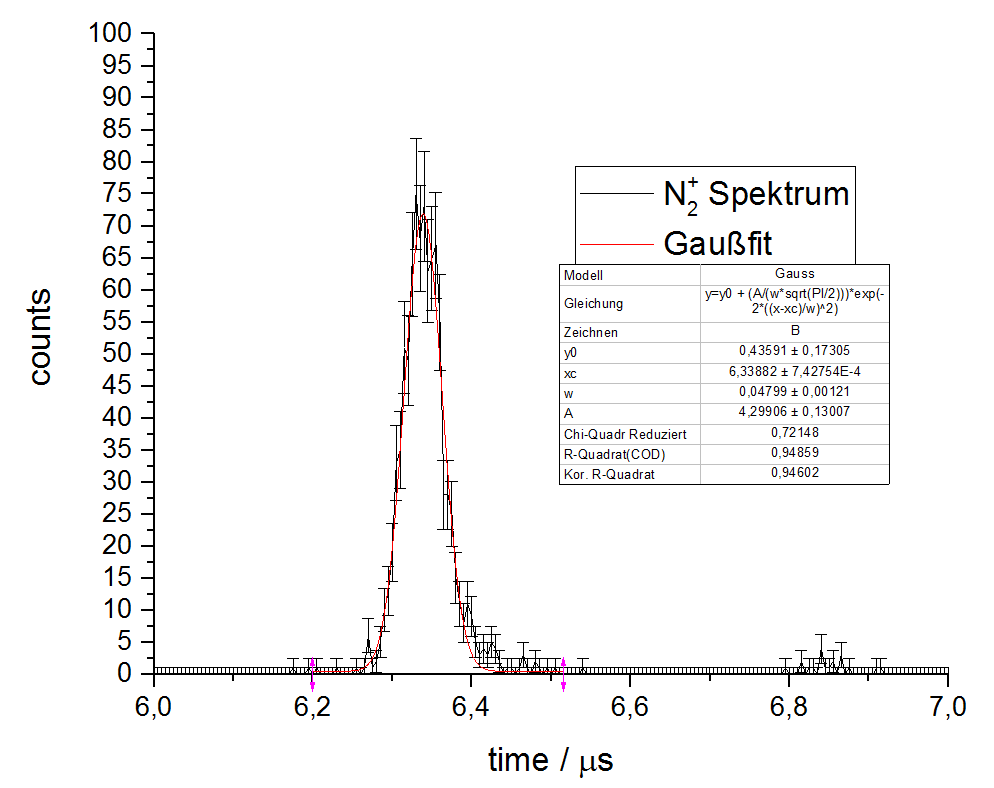
\includegraphics[width=0.6\columnwidth]{pics/N2}
					\caption{Flugzeitspektrum für N${}_2^+$-Ionen mit 100 Umläufen im Multireflektron. Der Fehler ist der statistische Fehler der Messwerte. Die durchgelegte Kurve ist ein fehlergewichteter Gaußfit.}
					\label{abb:N2}
				\end{figure}
				
				\begin{figure}[!h]
					\centering
					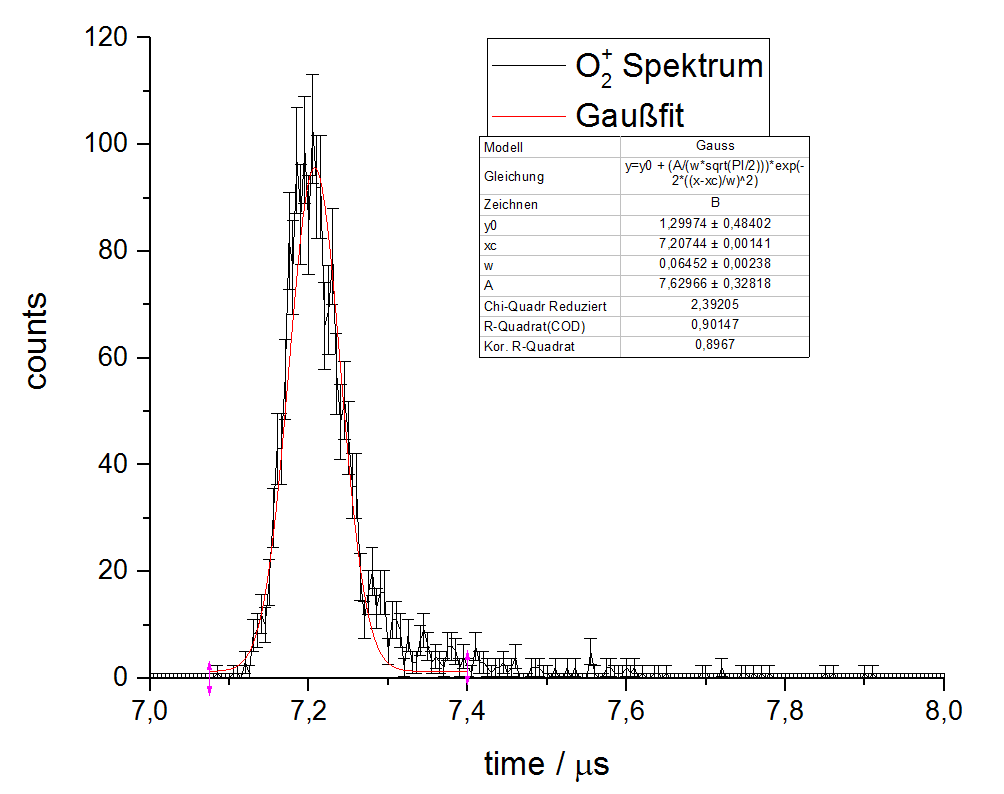
\includegraphics[width=0.6\columnwidth]{pics/O2}
					\caption{Flugzeitspektrum für O${}_2^+$-Ionen mit 100 Umläufen im Multireflektron. Der Fehler ist der statistische Fehler der Messwerte. Die durchgelegte Kurve ist ein fehlergewichteter Gaußfit.}
					\label{abb:O2}
				\end{figure}
				
				\begin{figure}[!h]
					\centering
					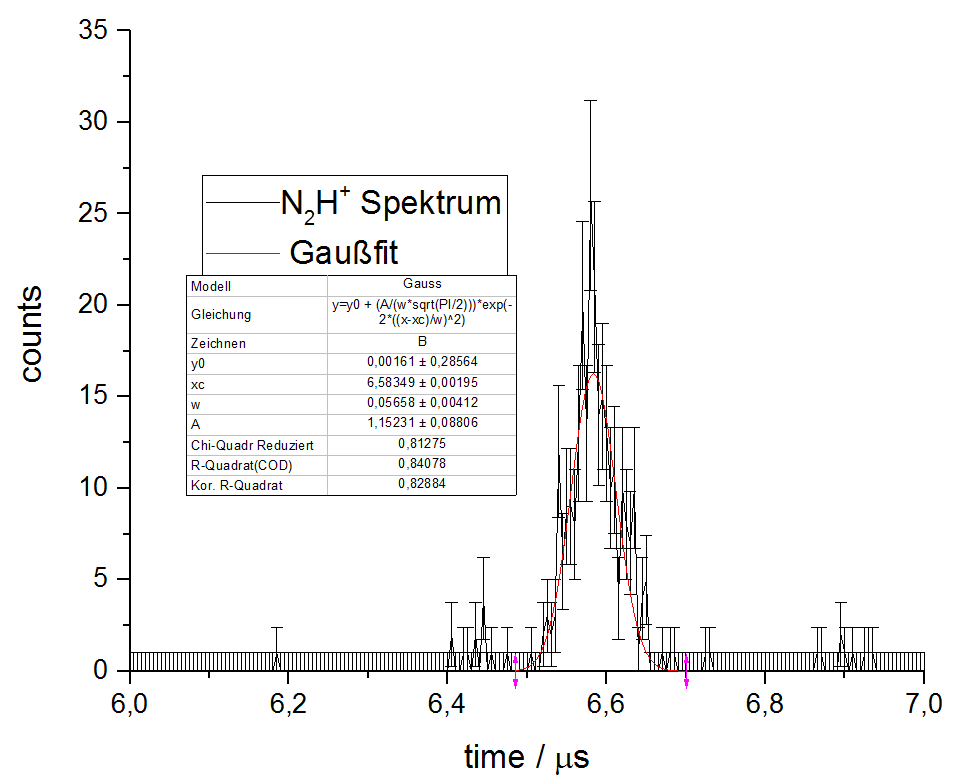
\includegraphics[width=0.6\columnwidth]{pics/N2H}
					\caption{Flugzeitspektrum für N${}_2$H$^+$-Ionen mit 100 Umläufen im Multireflektron. Der Fehler ist der statistische Fehler der Messwerte. Die durchgelegte Kurve ist ein fehlergewichteter Gaußfit.}
					\label{abb:N2H}
				\end{figure}
				\newpage
	
	\subsection{Massenbestimmung von N$_2^+$-Ionen}
		
		Für die berechneten Umlaufzeiten der drei angegebenen Ionen werden nun jeweils drei Spektren bei $100$ Umläufen im Multireflektron aufgenommen. Die Abb.\ref{abb:N2}-\ref{abb:N2H} sind beispielhaft die Spektren der ersten Messung versehen mit einem Gaußfit zur Bestimmung der Position des zeitlichen Peaks $\mu$, sowie dem Faktor $\sigma$, welcher über die Relation
		\begin{equation}
			b_\mathrm{FWHM} = 2 \sigma\sqrt{2 \ln 2}
		\end{equation}
		die Halbwertsbreite $b_\mathrm{FWHM}$ des Peaks angibt. Diese gibt den Fehler für die Positionsbestimmung des Peaks $\Delta t$ an. Die gemessene Positionen der Peaks im Flugzeitspektrum sind in Tab.\ref{tab:zeit} angegeben. Die Massen für O${}_2^+$- und N${}_2$H$^+$-Ionen werden als bekannt angenommen und es werden Werte aus der Literatur verwendet. Weiterhin wird angenommen, dass für die Fehlerrechnung der Fehler dieser Massen also $\Delta m_\mathrm{i} = 0$ gilt.
		\begin{table}[t]
			\centering
			\caption{Die gemessene Peakpostion $\mu$ für verschiedenen Ionensorten.}
			\begin{tabular}{c|c c c} 
				 & N$_2^+$ & O$_2^+$ & N$_2$H$^+$ \\
				 Nummer & $\mu\,/\,\mathrm{\mu s}$ & $\mu\,/\,\mathrm{\mu s}$ & $\mu\,/\,\mathrm{\mu s}$ \\ \hline
				 1 & $6,339$ & $7,807$ & $6,583$ \\
				 2 & $6,738$ & $7,208$ & $6,584$ \\
				 3 & $6,340$ & $7,208$ & $6,583$ 
			\end{tabular}
			\label{tab:zeit}
		\end{table}
		Aus diesen Werten lässt sich mit \eqref{eq:masse} und \eqref{eq:masse} die Masse von N$_2^+$ berechnen, wobei $t_1$, $t_2$, $m_1$, $m_2$ die Massen und Flugzeiten der bekannten Ionensorten sind. Weiterhin ist die Zeit $t$ ist die Summe aus der Zeit im Flugzeitspektrum $\mu$, der Zeit in Multireflektron $n\cdot t_\mathrm{U}$ und der Flugzeit von der Ionenquelle bis zum Reflektron, hier als $7\,\mathrm{\mu s}$ gemessen. Der Fehler für die gemessenen Massen ist nach der gaußschen Fehlerfortpflanzung berechnet (Formeln: siehe Anhang). Beides ist in Tab.\ref{tab:masse} angegeben. In der Abb.\ref{abb:masse} sind die Messwerte mit dem jeweiligen absoluten Massenfehler abgebildet. Die erste und die dritte errechnete Masse liegt jeweils weit unterhalb dem erwarteten Massenbereich von $28,05\,\mathrm{u}$. Bei der Messung Tab.\ref{tab:zeit} ist aufgefallen, dass die Peaks der Flugzeitspektren von gleichen Ionensorten bei verschiedenen Messungen weit auseinander liegen. Es ist also anzunehmen, dass bei der Aufnahme der Messdaten ein Fehler unterlaufen ist. Wahrscheinlich wurden die Schaltzeiten für das Reflektron, welche ebenfalls den Start der Datenaufnahme kennzeichnet, zwischen den Messungen falsch gesetzt, was zur Verschiebung der Peaks führte. Die Auswertung wird dennoch fortgesetzt, da die zweite Messung Ergebnisse in einem akzeptablen Massenbereich liefert.
				\begin{figure}[!h]
					\centering
					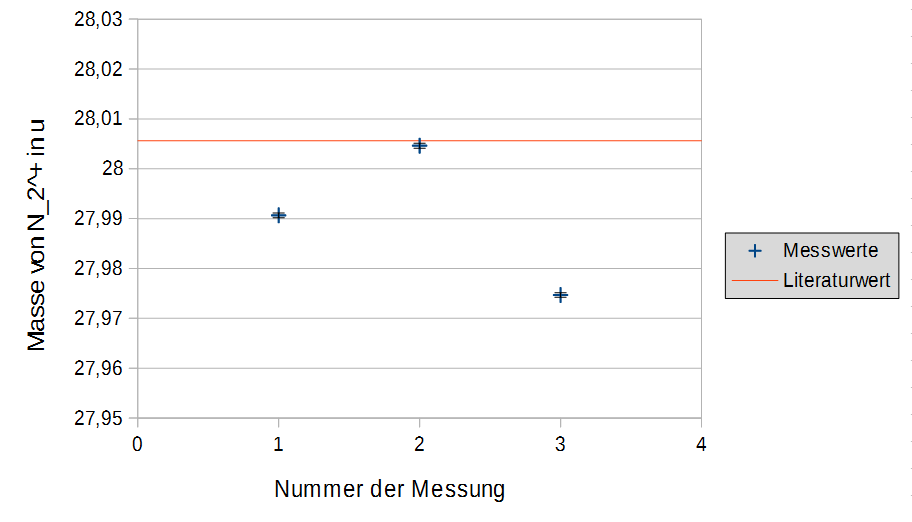
\includegraphics[width = 0.7\columnwidth]{pics/Masse}
					\caption{Experimentell errechnete Werte zur Bestimmung der Masse von N$_2^+$-Ionen. Jeder Messpunkt korrespondiert zu einer eigenden Kalibrierung. Die rote Makierung im Graphen repräsentiert den Literaturwert der Ionenmasse. Der Fehler ist durch gaußsche Fehlerfortpflanzung errechnet.}
					\label{abb:masse}
				\end{figure}
				
		
						\begin{table}[h]
					\centering
					\caption{Berechnete Massen $m$ für N$^+_2$-Ionen mit absoluten und relativen Fehler}
					\begin{tabular}{c|c c c} 
					
						Nummer & $m\,/\,\mathrm{u}$ & $\Delta m\,/\,\mathrm{u}$ & $\frac{\Delta m}{m}$ \\ \hline
						1 & $27,991$ & $4,89\cdot 10^{-4}$ & $1,75\cdot 10^{-5}$ \\
						2 & $28,004$ & $5,09\cdot 10^{-4}$ & $1,82\cdot 10^{-5}$ \\
						3 & $27,975$ & $4,43\cdot 10^{-4}$ & $1,58\cdot 10^{-5}$ 
					\end{tabular}
					\label{tab:masse}
				\end{table}
				\newpage

		\subsection{Bindungsenergie und Neutronenseparationsenergie}
		
		Mit der gemessenen Masse von $^{14}$N$^+_2$-Ionen und den Literaturwerten der Protonen-, Neutronenmasse lässt sich die, durch den Massendefekt verursachte, Diskrepanz zwischen der Ionenmasse und der Masse aller Kernteilchen des Ions bestimmen. Die Bindungsenergie $\mathrm{BE}$ ist dann gegeben über die Ruheenergie
			\begin{equation}
				\Delta E = \Delta m\cdot c^2
			\end{equation}
		Die berechneten Bindungsenergien sind in Tab.\ref{tab:bind} mit Vergleich zum Literaturwert aufgeführt. Da die gemessenen Massen i.A. niedriger waren als der Literaturwert ist hier ebenfalls eine Abweichung zu beobachten, jedoch zu höheren Bindungsenergien.
		\begin{table}[h]
			\centering
			\caption{Berechnete Bindungsenergien $\mathrm{BE}$ für $^{14}$N-Atome mit Vergleich zum Literaturwert.}
			\begin{tabular}{c|c} 
				
				Nummer & $\mathrm{BE}\,/\,\mathrm{MeV}$ \\ \hline
				1 & $111,38$ \\
				2 & $104,87$ \\
				3 & $118,81$ \\
				Literatur & $104,66$
			\end{tabular}
			\label{tab:bind}
		\end{table}
		Weiterhin lässt sich auch die Neutronenseparationsenergie $S_\mathrm{n}$ bzw. die Zwei-Neutronenseparationsenergie $S_\mathrm{2n}$ bestimmen. Es gilt
		\begin{align}
			S_\mathrm{n}(N,Z) = \mathrm{BE}(N,Z) - \mathrm{BE}(N-1,Z), \nonumber \\
			S_\mathrm{2n}(N,Z) = \mathrm{BE}(N,Z) - \mathrm{BE}(N-2,Z).
		\end{align}
		Es werden die Separationsenergien für $^{14}$N und $^{15}$N und die Zwei-Neutronenseparationsenergien für $^{16}$N und $^{14}$N bestimmt. Für die unbekannten Bindungsenergien werden Literaturwerte verwendet. Die errechneten Ergebnisse sind in Tab.\ref{tab:sep} aufgeführt. Weiterhin sind die Werte zur ersten und zweiten Messung abseits der erwarteten Literaturwerte.
				\begin{table}[h]
					\centering
					\caption{Berechnete Separationsenergien $S_\mathrm{n}$/$S_\mathrm{2n}$ für N-Atome mit Vergleich zum Literaturwert.}
					\begin{tabular}{c c|c} 
						Isotop & Nummer & $S_\mathrm{n}\,/\,\mathrm{MeV}$ \\ \hline
							     & 1 & $4,11$ \\
						$^{15}$N & 2 & $10,62$ \\
								 & 3 & $-3,32$ \\ \hline
						$^{15}$N & Literatur & $10,83$ \\ \hline
								 & 1 & $17,27$ \\
				 		$^{14}$N & 2 & $10,76$ \\
				 				 & 3 & $24,71$ \\ \hline
						$^{14}$N & Literatur & $10,56$ \\ \hline
					\end{tabular}
					\quad
					\begin{tabular}{c c|c} 
						Isotop & Nummer & $S_\mathrm{2n}\,/\,\mathrm{MeV}$ \\ \hline
								 & 1 & $6,60$ \\
						$^{16}$N & 2 & $13,11$ \\
								 & 3 & $-0,83$ \\ \hline
						$^{16}$N & Literatur & $13,32$ \\ \hline
								 & 1 & $37,32$ \\
						$^{14}$N & 2 & $30,81$ \\
								 & 3 & $44,75$ \\ \hline
						$^{14}$N & Literatur & $30,60$ \\ \hline
						\end{tabular}
					\label{tab:sep}
				\end{table}
				
				\subsection{Fazit}
			
			Es ist trotz einiger Abweichung der Messungen von den Literaturwerten gelungen die Prinzipien des Versuches gut nachzuvollziehen. Eine der Messreihen war sogar erfolgreich und lieferte einen Wert, welcher vergleichbar mit den Literaturangaben ist.
				
	\newpage
	\section{Anhang}
		\subsection{Fehlerrechnung}
		
		Die Fehlerrechnung für den absoluten Massenfehler $\Delta m$ ergibt sich durch gaußsche Fehlerfortpflanzung der Formel \eqref{eq:masse} und den Fehlerwerten von $t_1$,$t_2$ und $t$
		\begin{equation}
			\Delta m = \sqrt{\left(\frac{\partial m}{\partial t_1}\cdot \Delta t_1\right)^2+\left(\frac{\partial m}{\partial t_2}\cdot \Delta t_2\right)^2+\left(\frac{\partial m}{\partial t}\cdot \Delta t \right)^2}
		\end{equation}
		Die Ableitungen nach den Referenzmassen $m_1$ und $m_2$ werden als fehlerlos betrachtet, da deren Fehlerwert im Vergleich zu denen des Experimentes hinreichend klein sind. Die partiellen Ableitungen sind gegen durch
		\begin{align}
			\frac{\partial m}{\partial t_1} =& 2 \left(C_\mathrm{ToF}\cdot \Delta_\mathrm{ref}+\frac{\Sigma_\mathrm{ref}}{2}\right) \cdot \Delta_\mathrm{ref}\frac{t_2-t}{\left(t_1-t_2\right)^2} \nonumber \\
			\frac{\partial m}{\partial t_2} =& 2 \left(C_\mathrm{ToF}\cdot \Delta_\mathrm{ref}+\frac{\Sigma_\mathrm{ref}}{2}\right) \cdot \Delta_\mathrm{ref}\frac{t-t_1}{\left(t_1-t_2\right)^2} \\
			\frac{\partial m}{\partial t} =& 2 \left(C_\mathrm{ToF}\cdot \Delta_\mathrm{ref}+\frac{\Sigma_\mathrm{ref}}{2}\right) \cdot \Delta_\mathrm{ref}\frac{1}{\left(t_1-t_2\right)^2} \nonumber
		\end{align}

		\subsection{Quellen}
		\begin{enumerate}
			 \item Versuchsanleitung Reflektron, Ernst-Moritz-Arndt-Universität Greifswald, 04.11.15
		\end{enumerate}
\end{document}